% Options for packages loaded elsewhere
\PassOptionsToPackage{unicode}{hyperref}
\PassOptionsToPackage{hyphens}{url}
%
\documentclass[
]{article}
\usepackage{amsmath,amssymb}
\usepackage{lmodern}
\usepackage{iftex}
\ifPDFTeX
  \usepackage[T1]{fontenc}
  \usepackage[utf8]{inputenc}
  \usepackage{textcomp} % provide euro and other symbols
\else % if luatex or xetex
  \usepackage{unicode-math}
  \defaultfontfeatures{Scale=MatchLowercase}
  \defaultfontfeatures[\rmfamily]{Ligatures=TeX,Scale=1}
\fi
% Use upquote if available, for straight quotes in verbatim environments
\IfFileExists{upquote.sty}{\usepackage{upquote}}{}
\IfFileExists{microtype.sty}{% use microtype if available
  \usepackage[]{microtype}
  \UseMicrotypeSet[protrusion]{basicmath} % disable protrusion for tt fonts
}{}
\makeatletter
\@ifundefined{KOMAClassName}{% if non-KOMA class
  \IfFileExists{parskip.sty}{%
    \usepackage{parskip}
  }{% else
    \setlength{\parindent}{0pt}
    \setlength{\parskip}{6pt plus 2pt minus 1pt}}
}{% if KOMA class
  \KOMAoptions{parskip=half}}
\makeatother
\usepackage{xcolor}
\IfFileExists{xurl.sty}{\usepackage{xurl}}{} % add URL line breaks if available
\IfFileExists{bookmark.sty}{\usepackage{bookmark}}{\usepackage{hyperref}}
\hypersetup{
  pdftitle={Dehnbare Stoffe},
  pdfauthor={Justus Weyers \& Milena Mensching, Team 4},
  hidelinks,
  pdfcreator={LaTeX via pandoc}}
\urlstyle{same} % disable monospaced font for URLs
\usepackage[margin=1in]{geometry}
\usepackage{color}
\usepackage{fancyvrb}
\newcommand{\VerbBar}{|}
\newcommand{\VERB}{\Verb[commandchars=\\\{\}]}
\DefineVerbatimEnvironment{Highlighting}{Verbatim}{commandchars=\\\{\}}
% Add ',fontsize=\small' for more characters per line
\usepackage{framed}
\definecolor{shadecolor}{RGB}{248,248,248}
\newenvironment{Shaded}{\begin{snugshade}}{\end{snugshade}}
\newcommand{\AlertTok}[1]{\textcolor[rgb]{0.94,0.16,0.16}{#1}}
\newcommand{\AnnotationTok}[1]{\textcolor[rgb]{0.56,0.35,0.01}{\textbf{\textit{#1}}}}
\newcommand{\AttributeTok}[1]{\textcolor[rgb]{0.77,0.63,0.00}{#1}}
\newcommand{\BaseNTok}[1]{\textcolor[rgb]{0.00,0.00,0.81}{#1}}
\newcommand{\BuiltInTok}[1]{#1}
\newcommand{\CharTok}[1]{\textcolor[rgb]{0.31,0.60,0.02}{#1}}
\newcommand{\CommentTok}[1]{\textcolor[rgb]{0.56,0.35,0.01}{\textit{#1}}}
\newcommand{\CommentVarTok}[1]{\textcolor[rgb]{0.56,0.35,0.01}{\textbf{\textit{#1}}}}
\newcommand{\ConstantTok}[1]{\textcolor[rgb]{0.00,0.00,0.00}{#1}}
\newcommand{\ControlFlowTok}[1]{\textcolor[rgb]{0.13,0.29,0.53}{\textbf{#1}}}
\newcommand{\DataTypeTok}[1]{\textcolor[rgb]{0.13,0.29,0.53}{#1}}
\newcommand{\DecValTok}[1]{\textcolor[rgb]{0.00,0.00,0.81}{#1}}
\newcommand{\DocumentationTok}[1]{\textcolor[rgb]{0.56,0.35,0.01}{\textbf{\textit{#1}}}}
\newcommand{\ErrorTok}[1]{\textcolor[rgb]{0.64,0.00,0.00}{\textbf{#1}}}
\newcommand{\ExtensionTok}[1]{#1}
\newcommand{\FloatTok}[1]{\textcolor[rgb]{0.00,0.00,0.81}{#1}}
\newcommand{\FunctionTok}[1]{\textcolor[rgb]{0.00,0.00,0.00}{#1}}
\newcommand{\ImportTok}[1]{#1}
\newcommand{\InformationTok}[1]{\textcolor[rgb]{0.56,0.35,0.01}{\textbf{\textit{#1}}}}
\newcommand{\KeywordTok}[1]{\textcolor[rgb]{0.13,0.29,0.53}{\textbf{#1}}}
\newcommand{\NormalTok}[1]{#1}
\newcommand{\OperatorTok}[1]{\textcolor[rgb]{0.81,0.36,0.00}{\textbf{#1}}}
\newcommand{\OtherTok}[1]{\textcolor[rgb]{0.56,0.35,0.01}{#1}}
\newcommand{\PreprocessorTok}[1]{\textcolor[rgb]{0.56,0.35,0.01}{\textit{#1}}}
\newcommand{\RegionMarkerTok}[1]{#1}
\newcommand{\SpecialCharTok}[1]{\textcolor[rgb]{0.00,0.00,0.00}{#1}}
\newcommand{\SpecialStringTok}[1]{\textcolor[rgb]{0.31,0.60,0.02}{#1}}
\newcommand{\StringTok}[1]{\textcolor[rgb]{0.31,0.60,0.02}{#1}}
\newcommand{\VariableTok}[1]{\textcolor[rgb]{0.00,0.00,0.00}{#1}}
\newcommand{\VerbatimStringTok}[1]{\textcolor[rgb]{0.31,0.60,0.02}{#1}}
\newcommand{\WarningTok}[1]{\textcolor[rgb]{0.56,0.35,0.01}{\textbf{\textit{#1}}}}
\usepackage{graphicx}
\makeatletter
\def\maxwidth{\ifdim\Gin@nat@width>\linewidth\linewidth\else\Gin@nat@width\fi}
\def\maxheight{\ifdim\Gin@nat@height>\textheight\textheight\else\Gin@nat@height\fi}
\makeatother
% Scale images if necessary, so that they will not overflow the page
% margins by default, and it is still possible to overwrite the defaults
% using explicit options in \includegraphics[width, height, ...]{}
\setkeys{Gin}{width=\maxwidth,height=\maxheight,keepaspectratio}
% Set default figure placement to htbp
\makeatletter
\def\fps@figure{htbp}
\makeatother
\setlength{\emergencystretch}{3em} % prevent overfull lines
\providecommand{\tightlist}{%
  \setlength{\itemsep}{0pt}\setlength{\parskip}{0pt}}
\setcounter{secnumdepth}{-\maxdimen} % remove section numbering
\ifLuaTeX
  \usepackage{selnolig}  % disable illegal ligatures
\fi

\title{Dehnbare Stoffe}
\author{Justus Weyers \& Milena Mensching, Team 4}
\date{2022-11-17}

\begin{document}
\maketitle

\hypertarget{versuch-1}{%
\section{Versuch 1}\label{versuch-1}}

\hypertarget{ziel}{%
\subsection{Ziel}\label{ziel}}

Überprüfung der Anwendbarkeit des Hookeschen Modells auf ein Gummiband
durch Bestimmung der Federkonstante

\hypertarget{materialien}{%
\subsection{Materialien}\label{materialien}}

\begin{itemize}
\tightlist
\item
  Stativ
\item
  Gummiband
\item
  Gewichte
\item
  Maßband
\item
  Haken
\item
  Klebeband
\end{itemize}

\hypertarget{versuchsaufbau}{%
\subsection{Versuchsaufbau}\label{versuchsaufbau}}

\begin{itemize}
\tightlist
\item
  Aufstellung des Stativs, Befestigung am Tisch
\item
  Befestigung des Hakens am Stativ
\item
  Befestigung des Maßbandes am Stativ mit Hilfe von Klebeband
\item
  Aufhängung des Gummibandes am Haken
\item
  In das Gummiband werden die Gewichte gehängt
\end{itemize}

\begin{figure}
\centering
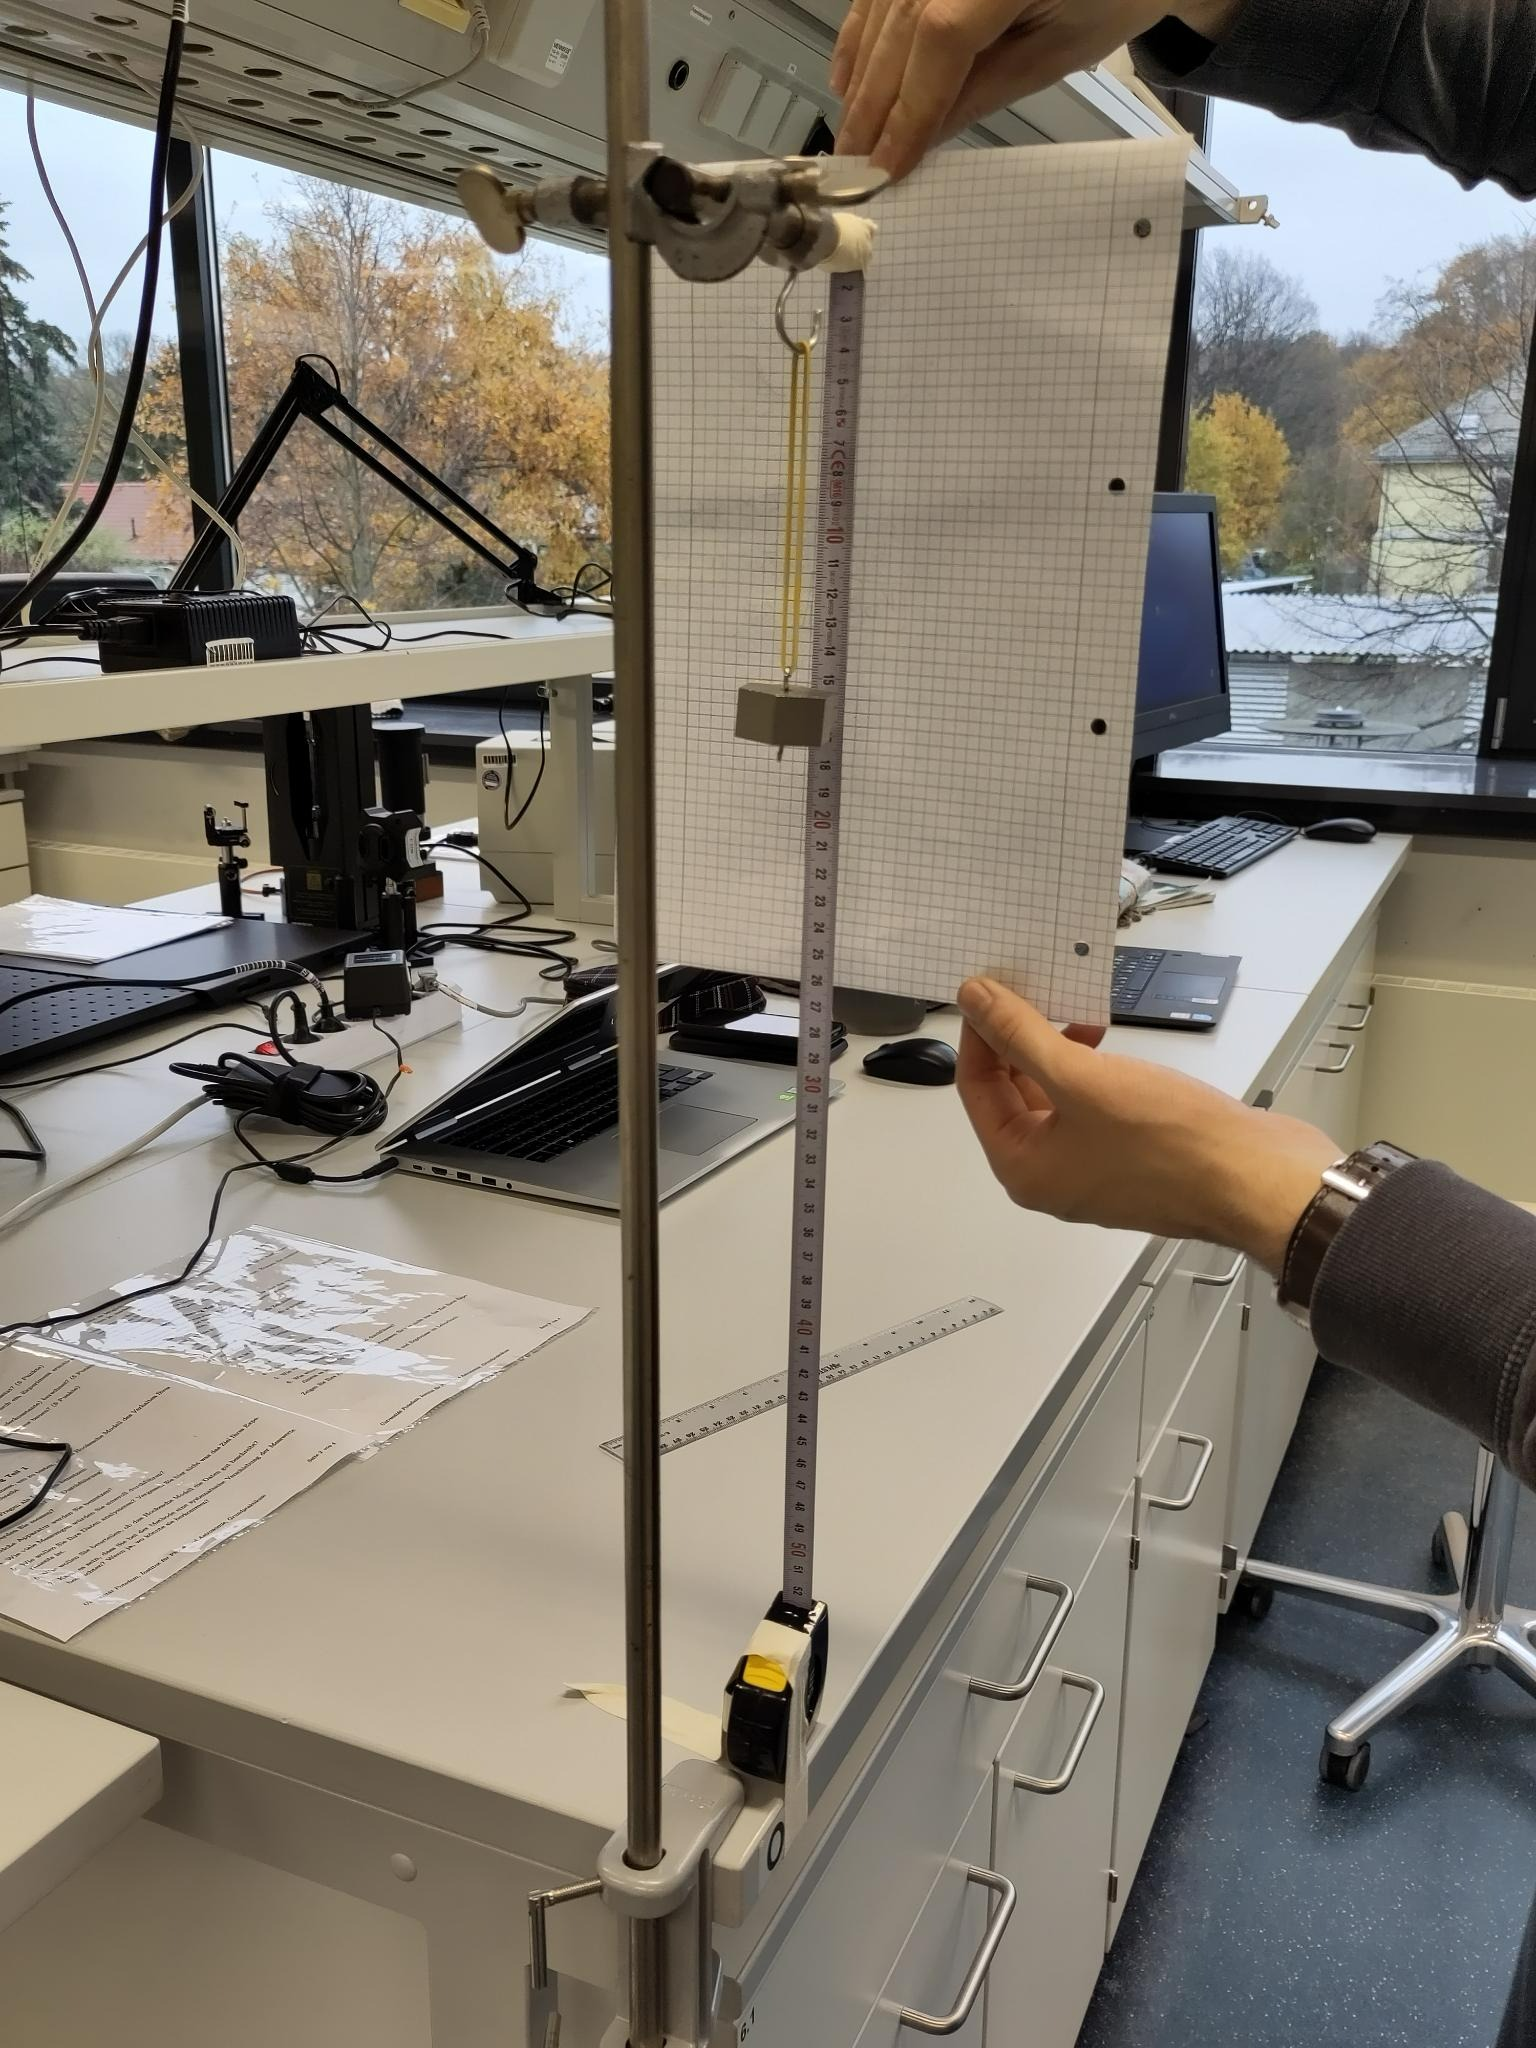
\includegraphics{C:/Users/milen/Documents/Studium/Physikpraktikum WiSe22,23/Laborbuch-im-Physikpraktikum/Laborbuch/Dehnbare Stoffe/Bilder/Versuch 1, Bild 2.jpeg}
\caption{Versuchsaufbau 1}
\end{figure}

\begin{figure}
\centering
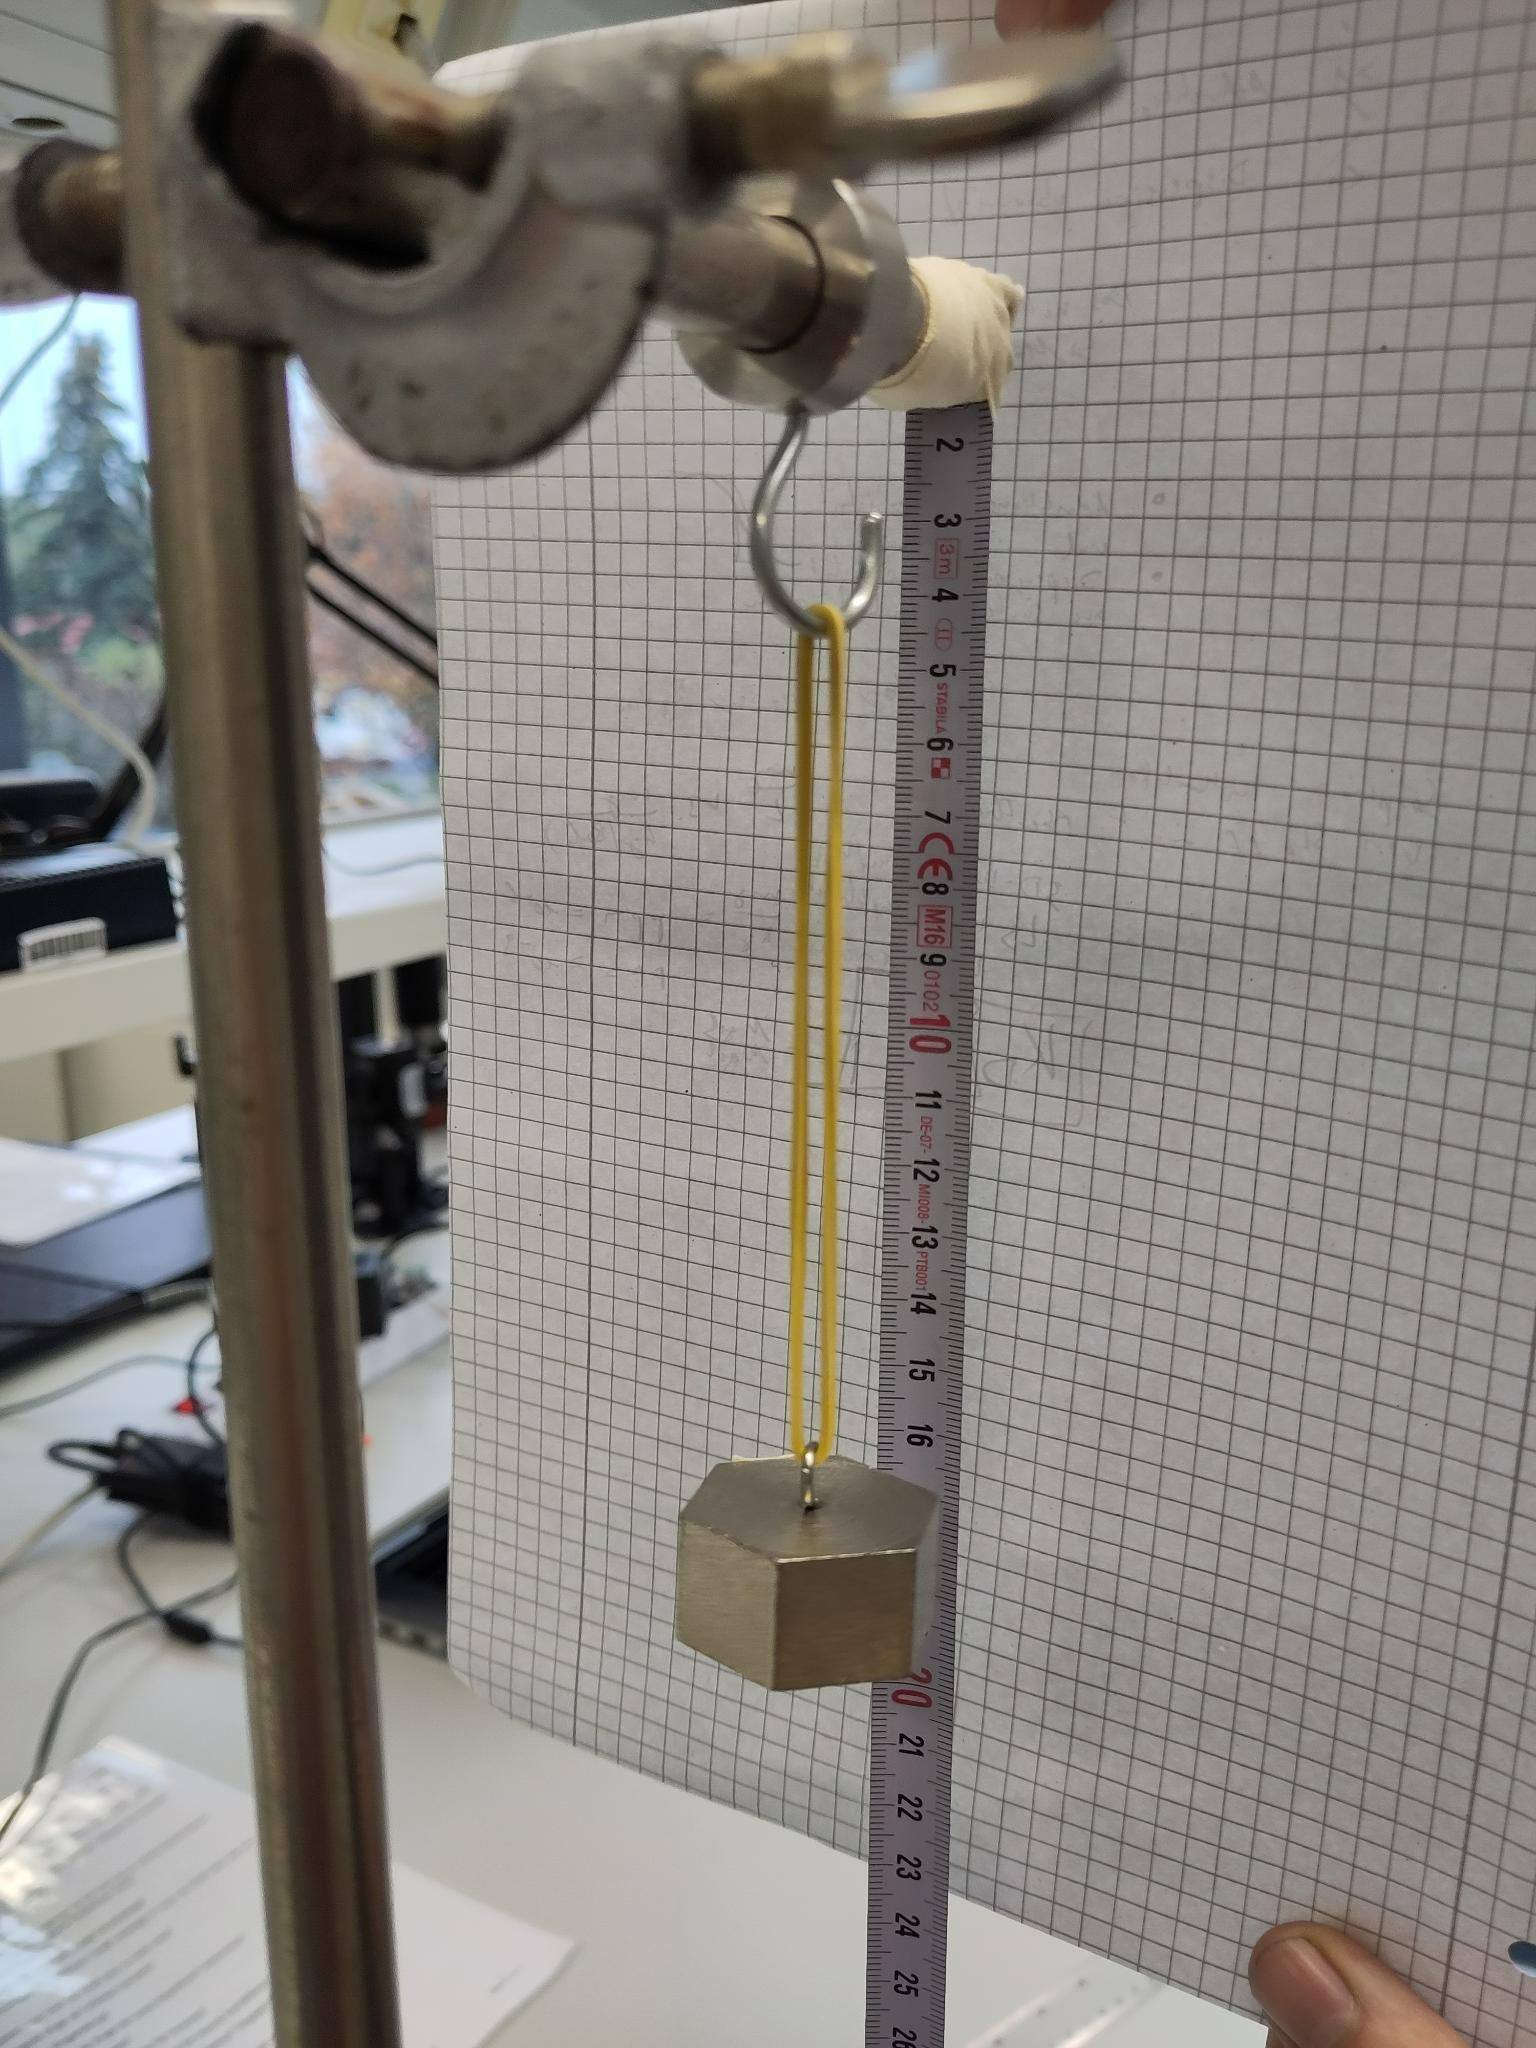
\includegraphics{C:/Users/milen/Documents/Studium/Physikpraktikum WiSe22,23/Laborbuch-im-Physikpraktikum/Laborbuch/Dehnbare Stoffe/Bilder/Versuch 1, Bild 1.jpeg}
\caption{Versuchsaufbau 1, Nahansicht}
\end{figure}

\hypertarget{durchfuxfchrung}{%
\subsection{Durchführung}\label{durchfuxfchrung}}

Die Gewichte werden gewogen und die Messunsicherheiten berechnet.
Gewichte:

\begin{Shaded}
\begin{Highlighting}[]
\NormalTok{Gewichte }\OtherTok{\textless{}{-}} \FunctionTok{read.csv}\NormalTok{(}\StringTok{"Gewichte.csv"}\NormalTok{, }\AttributeTok{sep=}\StringTok{";"}\NormalTok{, }\AttributeTok{dec=}\StringTok{","}\NormalTok{)}
\NormalTok{Gewichte[,}\FunctionTok{c}\NormalTok{(}\DecValTok{1}\NormalTok{,}\DecValTok{2}\NormalTok{)]}
\end{Highlighting}
\end{Shaded}

\begin{verbatim}
##        Name Masse..g.
## 1        5g       4.8
## 2  10g (2x)      10.0
## 3       20g      19.8
## 4       50g      49.9
## 5 100g (2x)      99.5
## 6      200g     198.5
\end{verbatim}

Messunsicherheiten:
\[u_m=\frac{a}{2\sqrt{3}}= \frac{0,0001kg}{2\sqrt{3}}=2,9*10^{-5}kg\]
Zunächst wird die Länge des Gummibandes ohne zusätzliches Gewicht
gemessen. Die Länge betrug 11,2 cm. Diese Länge muss später von allen
Messwerten abgezogen werden, um nur die Auslenkung aus dem Nullzustand
als Datensatz aufzunehmen.

Danach werden nacheinander verschiedene Gewichte an das Gummiband
gehängt und die entsprechende Auslenkung gemessen. Unsere Gruppe
entschied sich zunächst dafür, eine Messreihe mit Intervalen von 5g
durchzuführen. Nach den ersten 20 Messungen (100g) entschieden wir uns
dafür, die Intervalle auf 10g zu erhöhen, da wir zunächst den Aufwand
unterschätzten und Daten mit einem Abstand von 10g immer noch zur
Beurteilung der Federkonstante ausreichen.

Die Auslenkung wird am Maßband abgelesen (Messskala in mm). Dies
bedeutet eine Ungenauigket der Skala von:
\[u_{Skala}=\frac{a}{2\sqrt{6}}= \frac{0,001m}{2\sqrt{6}}=2,0*10^{-4}m\]

\hypertarget{fehlerquellen}{%
\subsection{Fehlerquellen}\label{fehlerquellen}}

Bei den Fehlerquellen ist zunächst der \textbf{personenbezogene
Ablesefehler} zu erwähnen. Diesen versuchten wir weitestgehend zu
eliminieren, indem nur eine Person eine vollständige Datenreihe
aufnahm.\\

Eine weitere Fehlerquelle kann die \textbf{Zeitabhängigkeit der
Auslenkung} sein. Ein Gummiband kann nach einer gewissen Zeit mehr
nachgeben, als bei der direkten Messung. Wir haben uns bemüht, die
Messungen sehr direkt und ohne Verzug vorzunehmen. Die Zeitanghängigkeit
haben wir jedoch nicht näher untersucht.\\

Besonders wichtig ist zu erwähnen, dass die Länge \(x_0\) am Anfang und
am Ende nicht übereinstimmten (11,2cm am Anfang zu 11,6cm am Ende). Dies
ist auf die \textbf{konstante Dehnung des Gummibandes} zurückzuführen
und wurde ebenfalls bei der Messung vernachlässigt.

\hypertarget{messung}{%
\subsection{Messung}\label{messung}}

Unsere Messergebnisse sind als csv-Datei abgespeichert:

\begin{Shaded}
\begin{Highlighting}[]
\NormalTok{Messreihe }\OtherTok{\textless{}{-}} \FunctionTok{read.csv}\NormalTok{(}\StringTok{"Messreihe.csv"}\NormalTok{, }\AttributeTok{sep=}\StringTok{";"}\NormalTok{, }\AttributeTok{dec=}\StringTok{","}\NormalTok{)}
\FunctionTok{colnames}\NormalTok{(Messreihe)}\OtherTok{=}\FunctionTok{c}\NormalTok{(}\StringTok{"Gewicht"}\NormalTok{, }\StringTok{"Auslenkung1"}\NormalTok{,  }\StringTok{"Auslenkung2"}\NormalTok{, }\StringTok{"a"}\NormalTok{, }\StringTok{"b"}\NormalTok{)}
\NormalTok{Messreihe[,}\FunctionTok{c}\NormalTok{(}\DecValTok{1}\NormalTok{,}\DecValTok{2}\NormalTok{)]}
\end{Highlighting}
\end{Shaded}

\begin{verbatim}
##    Gewicht Auslenkung1
## 1        0        11.2
## 2        5        13.0
## 3       10        13.3
## 4       15        13.5
## 5       20        13.6
## 6       25        13.8
## 7       30        13.8
## 8       35        13.9
## 9       40        14.0
## 10      45        14.1
## 11      50        14.0
## 12      55        14.1
## 13      60        14.2
## 14      65        14.3
## 15      70        14.4
## 16      75        14.5
## 17      80        14.5
## 18      85        14.6
## 19      90        14.6
## 20      95        14.7
## 21     100        14.8
## 22     110        15.1
## 23     120        15.3
## 24     130        15.4
## 25     140        15.6
## 26     150        15.8
## 27     160        16.0
## 28     170        16.4
## 29     180        16.6
## 30     190        16.9
## 31     200        17.3
## 32     210        17.5
## 33     220        17.8
## 34     230        18.2
## 35     240        18.5
## 36     250        18.9
## 37     260        19.3
## 38     270        19.8
## 39     280        20.0
## 40     290        20.3
## 41     300        20.9
## 42     310        21.2
## 43     320        21.5
## 44     330        22.0
## 45     340        22.3
## 46     350        22.7
## 47     360        23.0
## 48     370        23.3
## 49     380        23.6
## 50     390        23.9
## 51     400        24.5
## 52     410        24.7
## 53     420        25.0
## 54     430        25.2
## 55     440        25.5
## 56     450        25.7
## 57     460        26.1
## 58     470        26.2
## 59     480        26.5
## 60     490        26.8
\end{verbatim}

\hypertarget{auswertung}{%
\subsection{Auswertung}\label{auswertung}}

Zur besseren Interpretation der Messergebnisse wird die Anfangshöhe des
Gummibandes als Nullauslenkung \(x_0\) definiert und von den anderen
Messwerten subtrahiert. Da die wirkende Kraft die Gewichtskraft
\(F=m*g\) ist gilt folgende Formel:

\[F = m * g = D*x\] \[\rightarrow D =\frac{m*g}{x}\] Die Unsicherheit
ergibt sich daher aus folgender Formel:

\[u_D=\sqrt{(\frac{\partial{D}}{\partial{m}}*u_m)^2+(\frac{\partial{D}}{\partial{x}}*u_x)^2}\]
Mit: \[\frac{\partial{D}}{\partial{m}} = \frac{g}{x}\]
\[\frac{\partial{D}}{\partial{x}} = -\frac{m*g}{x^2}\]
\[u_D=\sqrt{(\frac{g}{x}*u_m)^2+(-\frac{m*g}{x^2}*u_x)^2}\]

\begin{Shaded}
\begin{Highlighting}[]
\CommentTok{\# Erdbeschleunigung}
\NormalTok{g }\OtherTok{=} \FloatTok{9.81} \CommentTok{\#m/s\^{}2}
\NormalTok{u\_m }\OtherTok{=} \FloatTok{2.9}\SpecialCharTok{*}\DecValTok{10}\SpecialCharTok{**}\NormalTok{(}\SpecialCharTok{{-}}\DecValTok{5}\NormalTok{) }\CommentTok{\#kg}
\NormalTok{u\_x }\OtherTok{=} \FloatTok{2.0}\SpecialCharTok{*}\DecValTok{10}\SpecialCharTok{**}\NormalTok{(}\SpecialCharTok{{-}}\DecValTok{4}\NormalTok{) }\CommentTok{\#m}

\CommentTok{\# Daten einlesen}
\NormalTok{Messreihe }\OtherTok{\textless{}{-}} \FunctionTok{read.csv}\NormalTok{(}\StringTok{"Messreihe.csv"}\NormalTok{, }\AttributeTok{sep=}\StringTok{";"}\NormalTok{, }\AttributeTok{dec=}\StringTok{","}\NormalTok{)}
\FunctionTok{colnames}\NormalTok{(Messreihe)}\OtherTok{=}\FunctionTok{c}\NormalTok{(}\StringTok{"Gewicht"}\NormalTok{, }\StringTok{"Auslenkung1"}\NormalTok{,  }\StringTok{"Auslenkung2"}\NormalTok{, }\StringTok{"a"}\NormalTok{, }\StringTok{"b"}\NormalTok{)}

\CommentTok{\# Nullwerte abziehen}
\CommentTok{\# Messreihe$Auslenkung1 \textless{}{-} Messreihe$Auslenkung1 {-} 11.2}

\CommentTok{\# Einheitenrechnung}
\CommentTok{\# Messreihe$Gewicht \textless{}{-} Messreihe$Gewicht/1000 \#kg}
\CommentTok{\# Messreihe[, c(2,3)] \textless{}{-}  Messreihe[, c(2,3)]/100 \#m}

\CommentTok{\# Testplot}
\CommentTok{\# plot(x=Messreihe$Auslenkung2, y=Messreihe$Gewicht, }
\CommentTok{\#      ylim=c(0,500),}
\CommentTok{\#      xlim=c(0,50))}
\CommentTok{\# points(x=Messreihe$Auslenkung1, y=Messreihe$Gewicht)}

\CommentTok{\# Subset}
\NormalTok{Messreihe1 }\OtherTok{\textless{}{-}}\NormalTok{ Messreihe[, }\FunctionTok{c}\NormalTok{(}\DecValTok{1}\NormalTok{,}\DecValTok{2}\NormalTok{)]}
\NormalTok{Messreihe1}\SpecialCharTok{$}\NormalTok{Kraft }\OtherTok{\textless{}{-}}\NormalTok{ Messreihe1}\SpecialCharTok{$}\NormalTok{Gewicht }\SpecialCharTok{*}\NormalTok{ g}

\NormalTok{unsicherheit\_funktion }\OtherTok{\textless{}{-}} \ControlFlowTok{function}\NormalTok{(x,m)\{}
 
  \FunctionTok{return}\NormalTok{( }\FunctionTok{sqrt}\NormalTok{( ((g}\SpecialCharTok{/}\NormalTok{x)}\SpecialCharTok{*}\NormalTok{u\_m)}\SpecialCharTok{**}\DecValTok{2} \SpecialCharTok{+}\NormalTok{ ((}\SpecialCharTok{{-}}\NormalTok{m}\SpecialCharTok{*}\NormalTok{g}\SpecialCharTok{/}\NormalTok{x}\SpecialCharTok{**}\DecValTok{2}\NormalTok{)}\SpecialCharTok{*}\NormalTok{u\_x)}\SpecialCharTok{**}\DecValTok{2}\NormalTok{ ))}
\NormalTok{\}}

\NormalTok{Messreihe1}\SpecialCharTok{$}\NormalTok{u\_Federkonstante }\OtherTok{\textless{}{-}} \FunctionTok{unsicherheit\_funktion}\NormalTok{(}\AttributeTok{x=}\NormalTok{Messreihe1}\SpecialCharTok{$}\NormalTok{Auslenkung1,}\AttributeTok{m=}\NormalTok{Messreihe1}\SpecialCharTok{$}\NormalTok{Gewicht)}

\NormalTok{Messreihe1}\SpecialCharTok{$}\NormalTok{Federkonstante }\OtherTok{\textless{}{-}}\NormalTok{ Messreihe1}\SpecialCharTok{$}\NormalTok{Kraft}\SpecialCharTok{/}\NormalTok{Messreihe1}\SpecialCharTok{$}\NormalTok{Auslenkung1}

\FunctionTok{plot}\NormalTok{(}\AttributeTok{x=}\NormalTok{Messreihe1}\SpecialCharTok{$}\NormalTok{Auslenkung1, }\AttributeTok{y=}\NormalTok{Messreihe1}\SpecialCharTok{$}\NormalTok{Federkonstante)}
\end{Highlighting}
\end{Shaded}

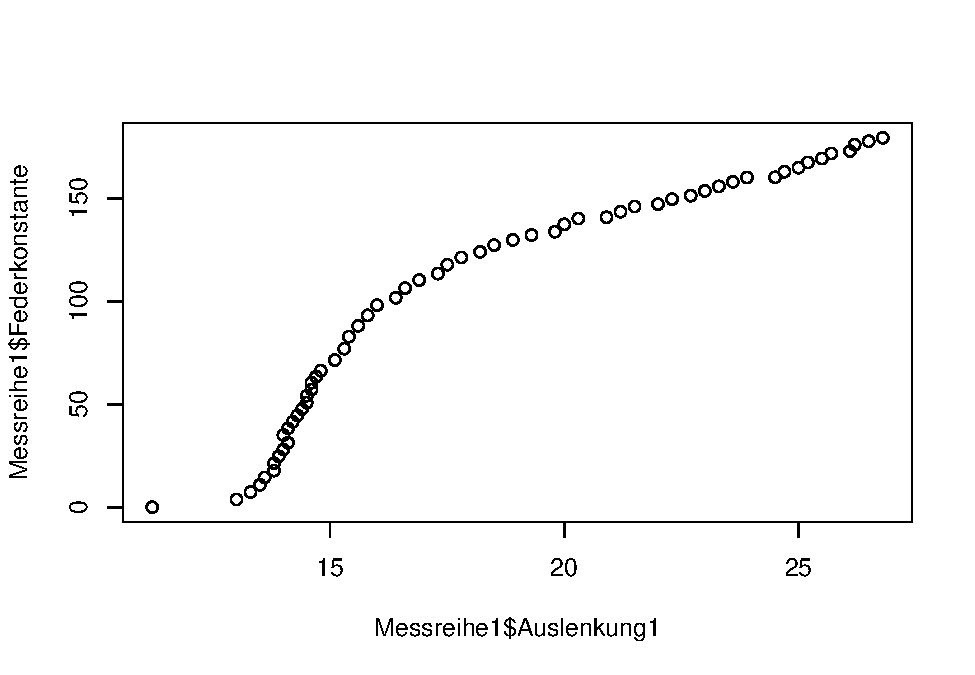
\includegraphics{DehnbareStoffe_files/figure-latex/unnamed-chunk-3-1.pdf}

\begin{Shaded}
\begin{Highlighting}[]
\FunctionTok{plot}\NormalTok{(}\AttributeTok{x=}\NormalTok{Messreihe1}\SpecialCharTok{$}\NormalTok{Auslenkung1, }\AttributeTok{y=}\NormalTok{Messreihe1}\SpecialCharTok{$}\NormalTok{Kraft)}
\end{Highlighting}
\end{Shaded}

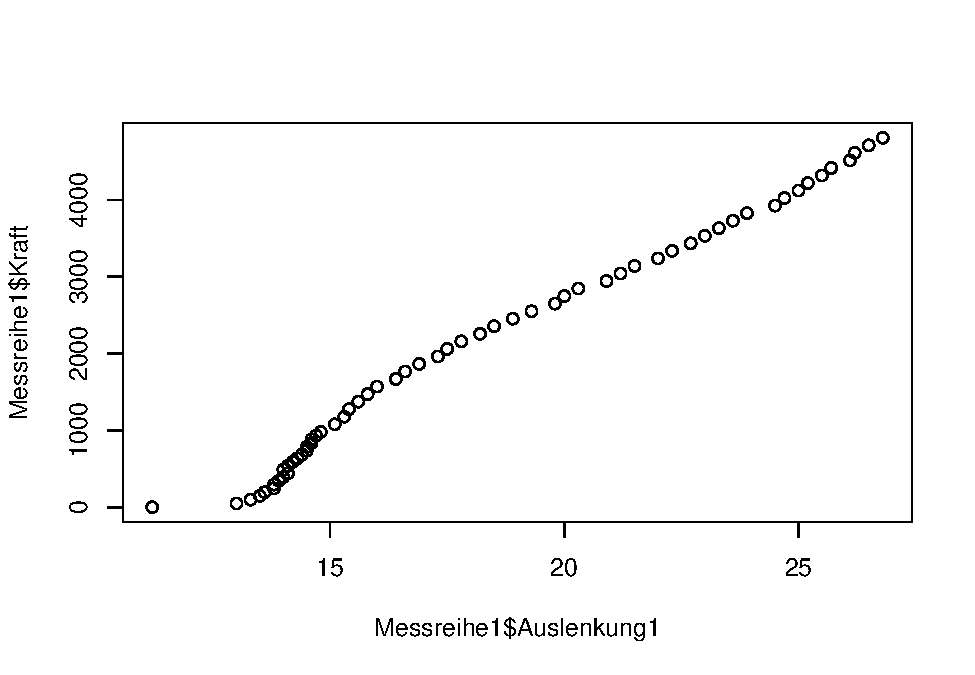
\includegraphics{DehnbareStoffe_files/figure-latex/unnamed-chunk-3-2.pdf}

\hypertarget{interpretation}{%
\subsection{Interpretation}\label{interpretation}}

\hypertarget{versuch-2}{%
\section{Versuch 2}\label{versuch-2}}

\hypertarget{ziel-1}{%
\subsection{Ziel}\label{ziel-1}}

Untersuchung der Fragestellung, ob sich der Zusammenhang zwischen Kraft
und Auslenkung verändert, wenn man die Angrifffskraft auf einen Strang
des Gummibandes anstatt auf zwei verteilt.

Eine Hypothese ist, dass die Auslenkung bei gleicher Gewichtskraft
doppelt so hoch ist, weil die Kraft auf nur einen Strang wirkt.

\hypertarget{materialien-1}{%
\subsection{Materialien}\label{materialien-1}}

\begin{itemize}
\tightlist
\item
  Stativ
\item
  Gummiband
\item
  Gewichte
\item
  Maßband
\item
  Haken
\item
  Klebeband
\item
  Schere
\end{itemize}

\hypertarget{versuchsaufbau-1}{%
\subsection{Versuchsaufbau}\label{versuchsaufbau-1}}

\begin{itemize}
\tightlist
\item
  Analog zu Versuch 1, aber das Gummiband wurde vorher mit einer Schere
  zerschnitten und durch geknotete Schlaufen an Haken und Gewicht
  befestigt.
\end{itemize}

\begin{figure}
\centering
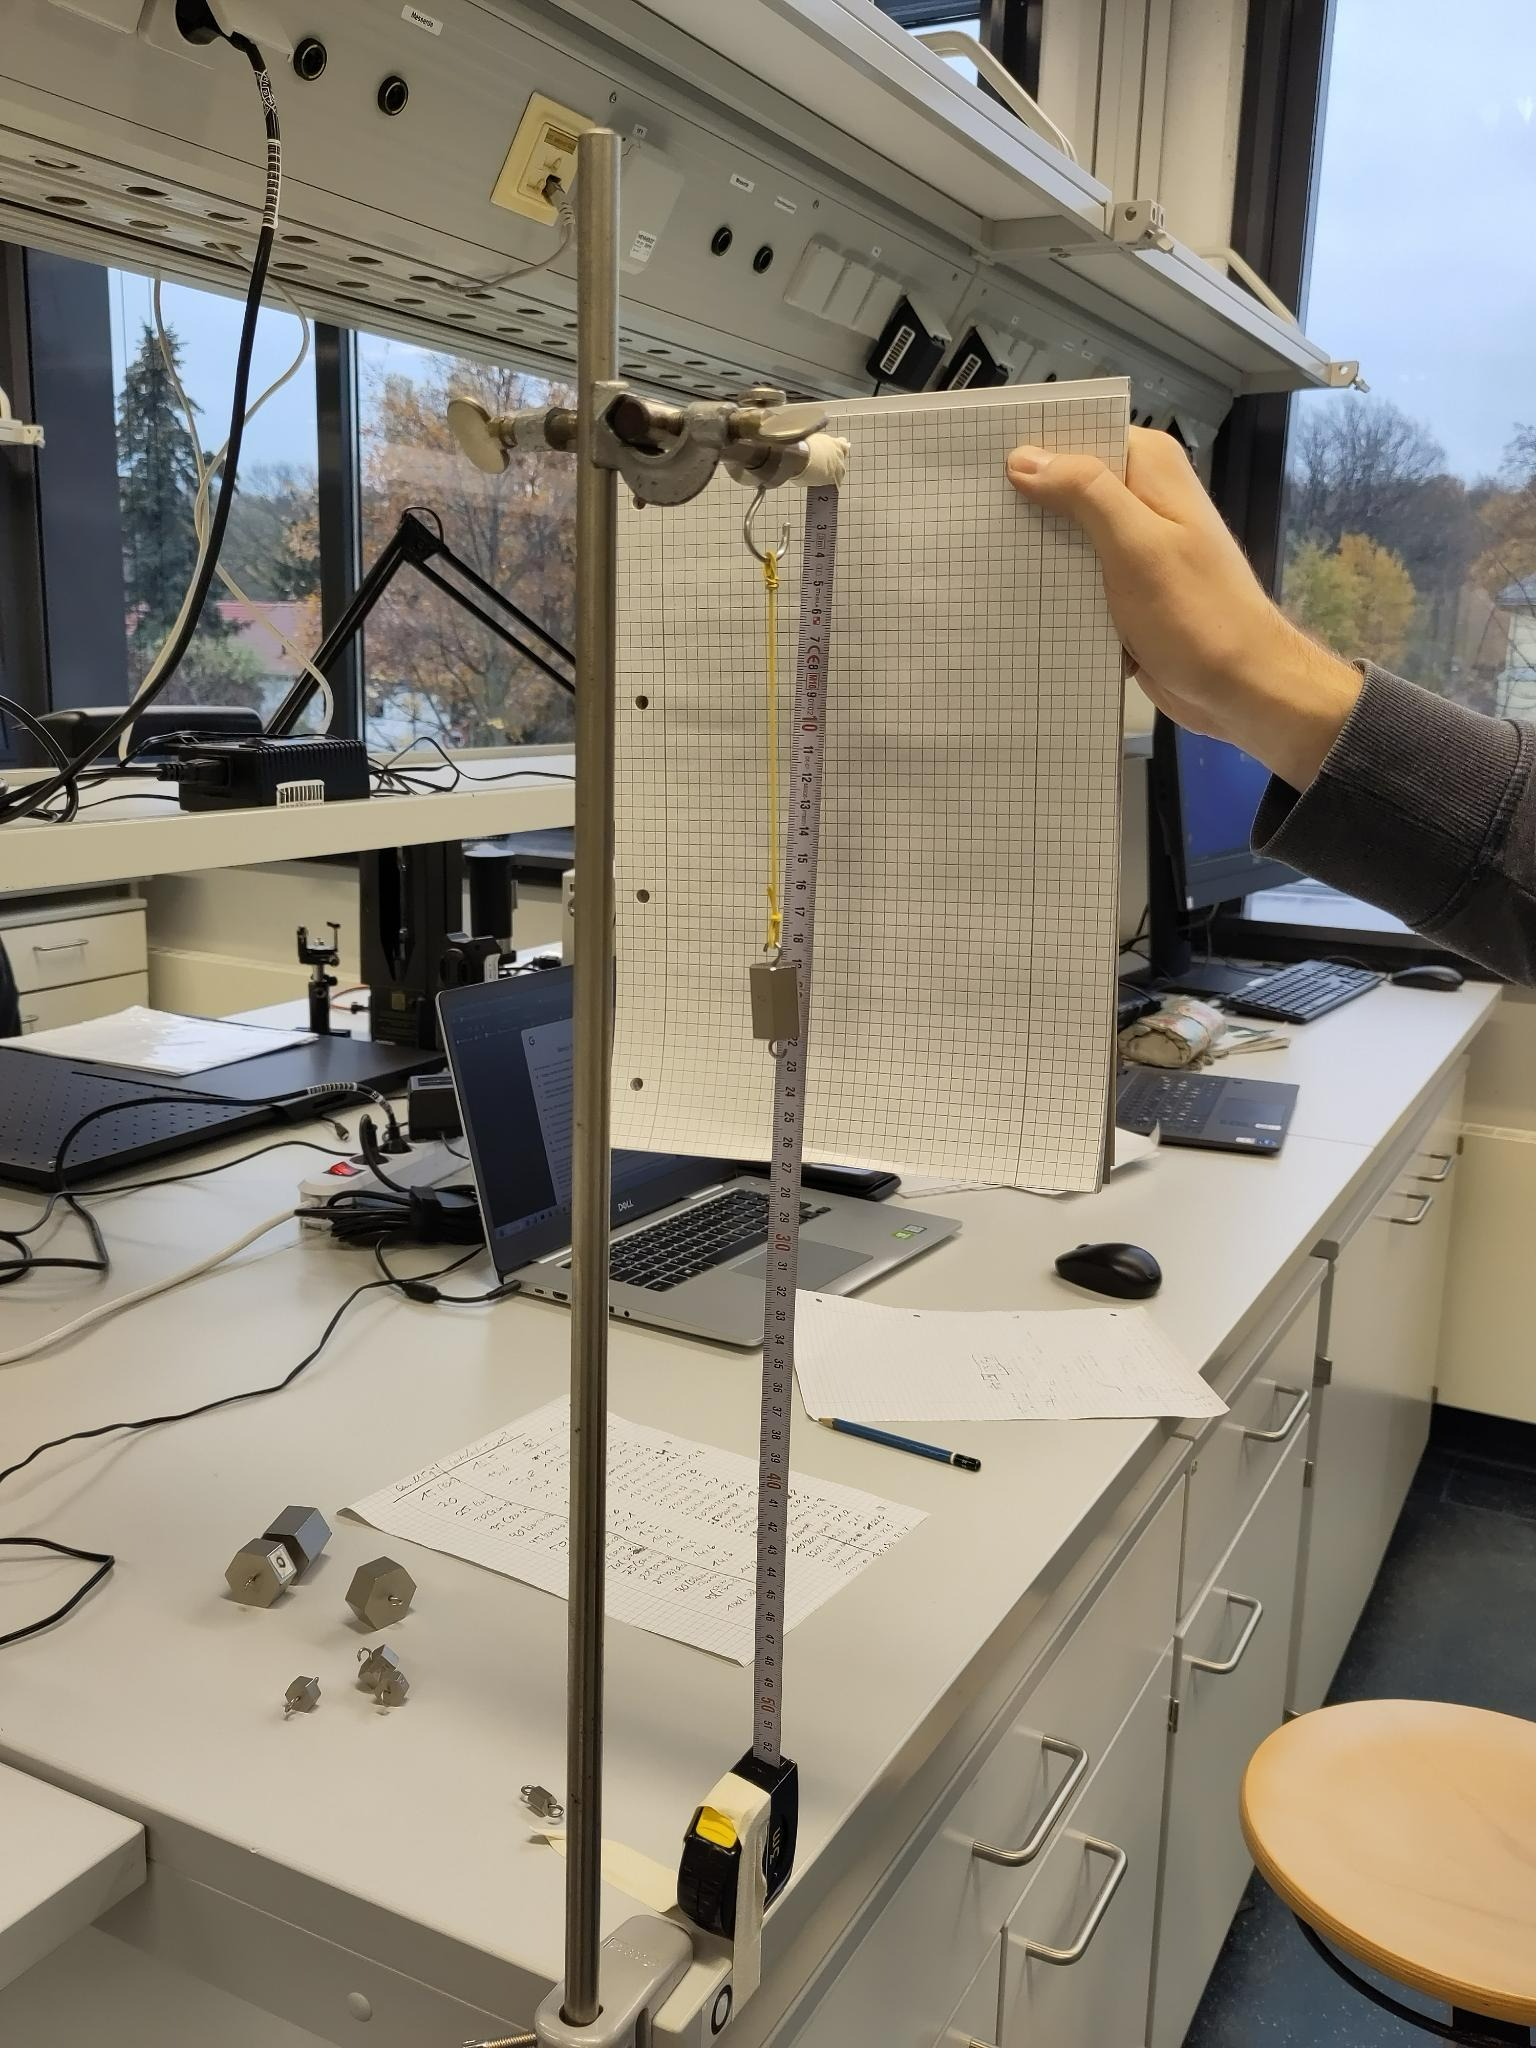
\includegraphics{C:/Users/milen/Documents/Studium/Physikpraktikum WiSe22,23/Laborbuch-im-Physikpraktikum/Laborbuch/Dehnbare Stoffe/Bilder/Versuch 2, Bild 2.jpeg}
\caption{Versuchsaufbau 2}
\end{figure}

\begin{figure}
\centering
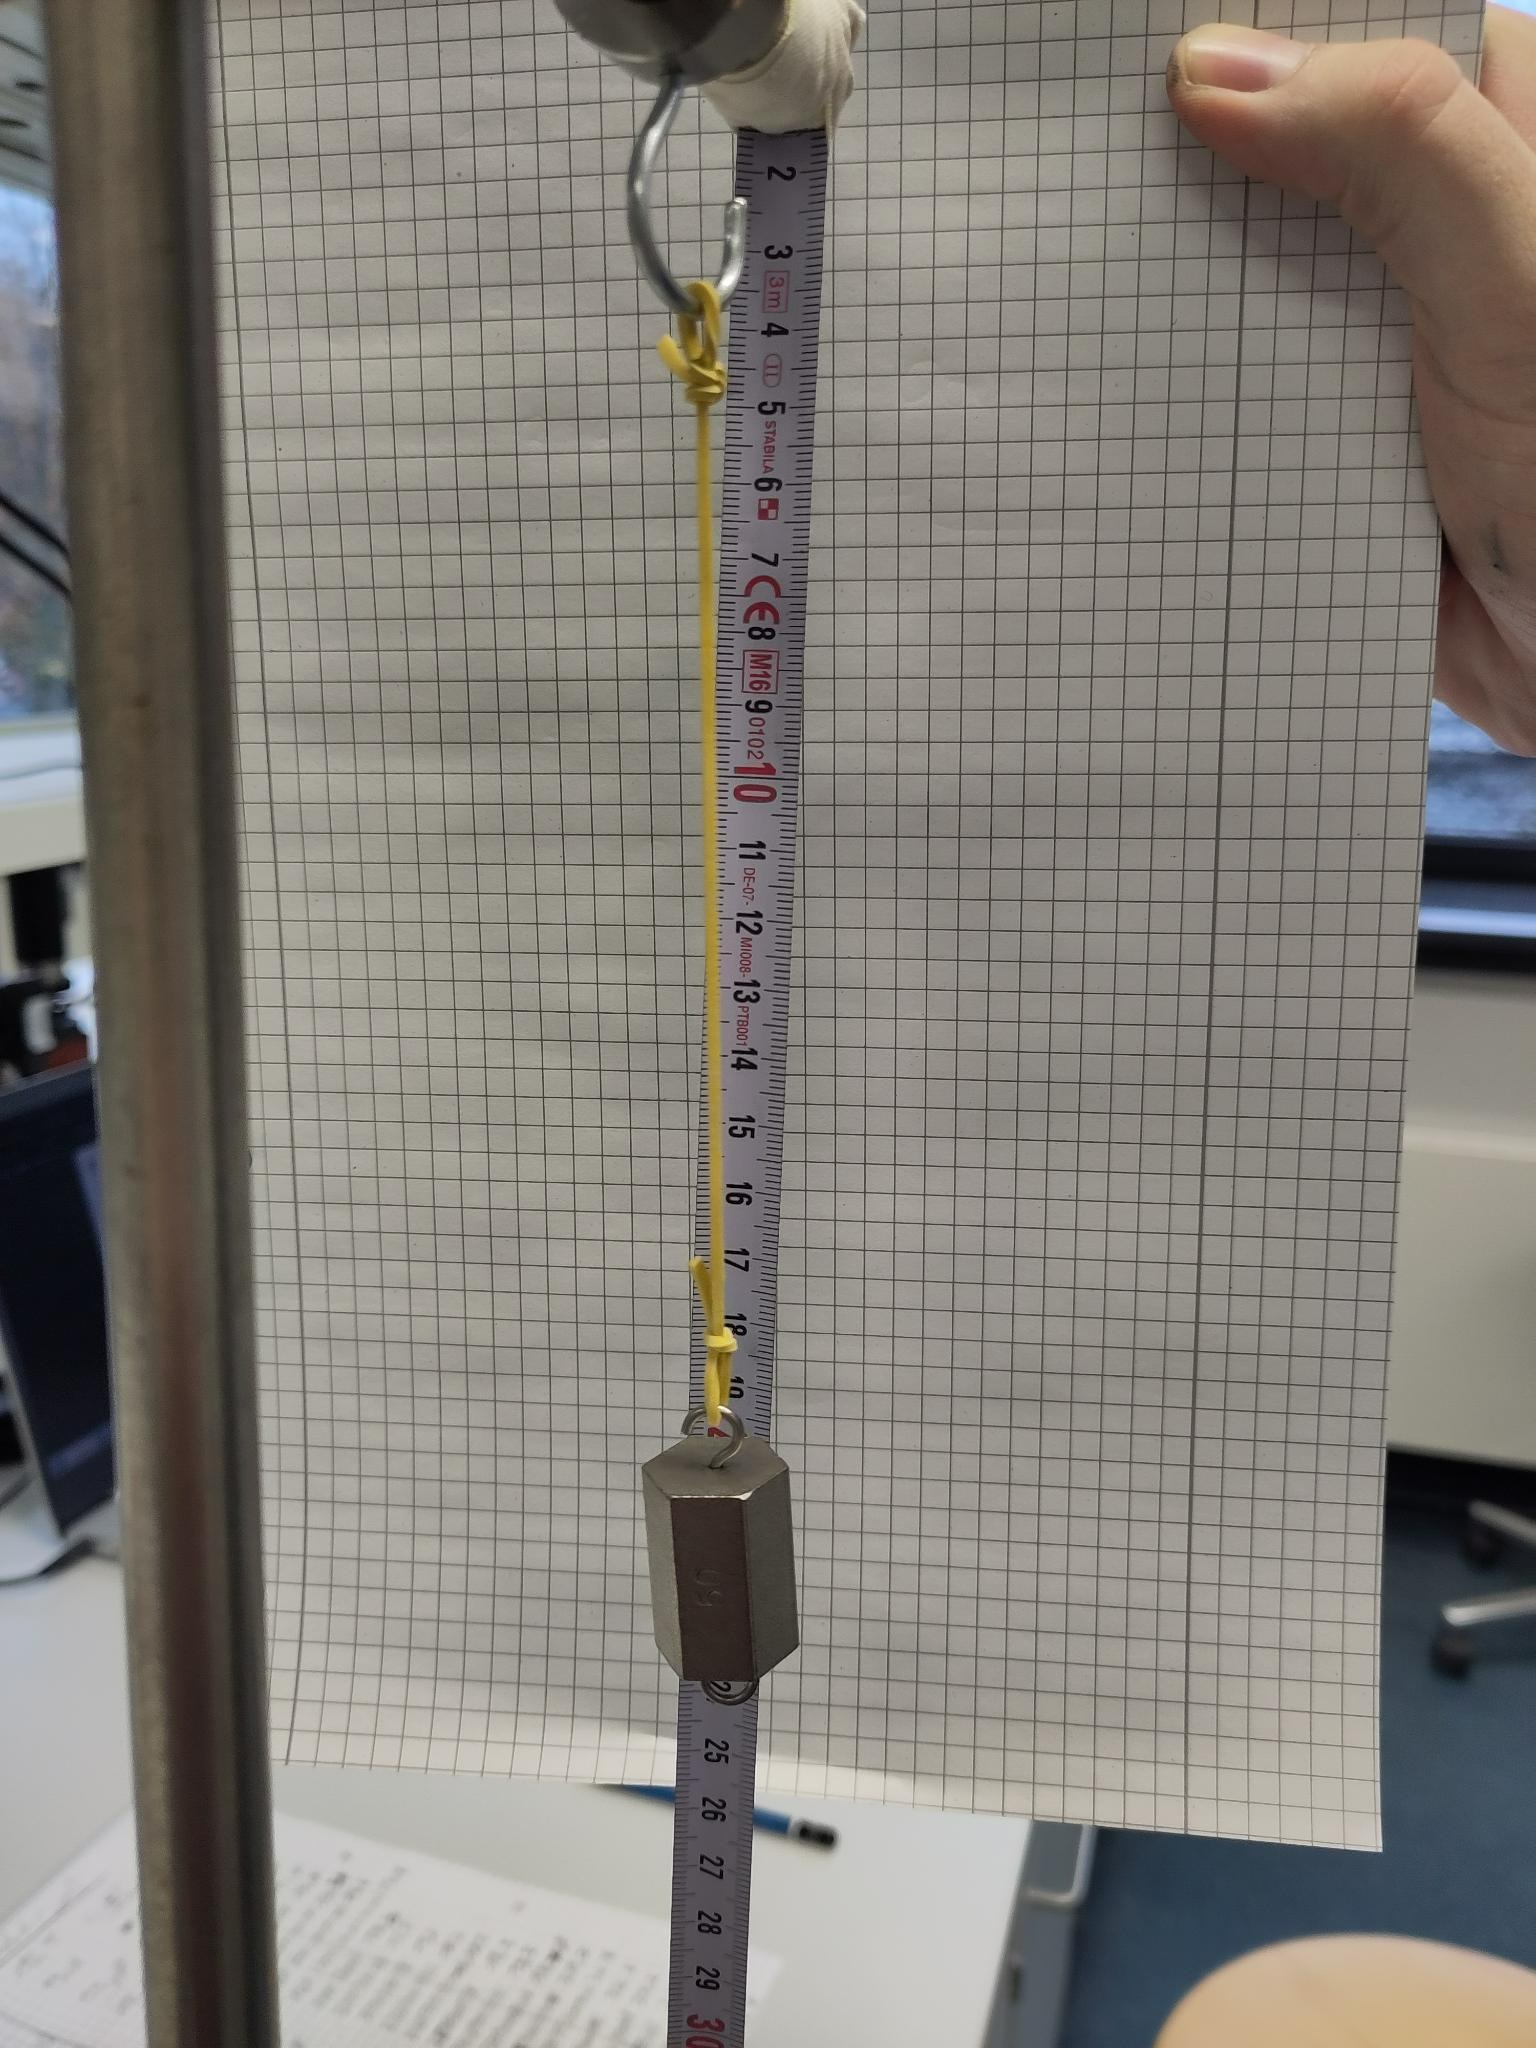
\includegraphics{C:/Users/milen/Documents/Studium/Physikpraktikum WiSe22,23/Laborbuch-im-Physikpraktikum/Laborbuch/Dehnbare Stoffe/Bilder/Versuch 2, Bild 1.jpeg}
\caption{Versuchsaufbau 2, Nahansicht}
\end{figure}

\hypertarget{durchfuxfchrung-1}{%
\subsection{Durchführung}\label{durchfuxfchrung-1}}

Analog zu Versuch 1. Wir haben uns dafür entschieden bis zur Marke von
100g in 5g - Intervallen und danach in 10g- Schriiten zu messen, um die
Daten mit den Daten aus der ersten Versuchsreihe gut vergleichen können.
Da das Band allerdings viel stärker durch das Anbringen von Gewicht
gedehnt wurde, konnten wir ab 360g keine Messungewn mehr durchführen, da
die Gewichte durch ihre Länge anfingen am Tisch aufzuliegen und so die
Normalkraft die Gewichtskraft verfälscht hätte. Stattdessen haben wir
den aus platztechnisch noch gut messbaren Wert für 400g genommen und den
Rest der Tabelle nicht ausgefüllt. \(x_0\) lag bei uns in diesem Fall
bei 15,8cm.

\hypertarget{messung-1}{%
\subsection{Messung}\label{messung-1}}

\hypertarget{auswertung-1}{%
\subsection{Auswertung}\label{auswertung-1}}

\hypertarget{interpretation-1}{%
\subsection{Interpretation}\label{interpretation-1}}

\end{document}
